\chapter{Literature Review} \label{cha:litrev}
In this chapter we will explore the theoretical background of our work, including research conducted on problems caused by current Android permission models, other solutions found and related work, and applications of trust transitivity in other domains.

\section{The Android Permission Model}
The Android permission model has been developed and updated since the introduction of Android as an operating system. We will examine the theoretical applications of how the permission model is expected to provide privacy and security in this section. 

\subsection{Application Security and Privacy}
Android runs on a Linux kernel. Each application is allocated aUID scene, sandboing, communicating between sandboxes, etc.
\smallskip


The Android OS allows users to install both free and paid third party Java applications through markets such as Google Play. As discussed Android applications do not go through a review process to measure compliance to guidelines, although most competitors including iOS, Windows and RIM do. Access to sensitive resources, also known as "permissions" are provided through the API, and applications are allowed to define their own extra permissions in addition to the 134 core permissions provided by Android. However this research will not be concerned with these third-party defined permissions\cite{a}.

%\begin{figure}
%  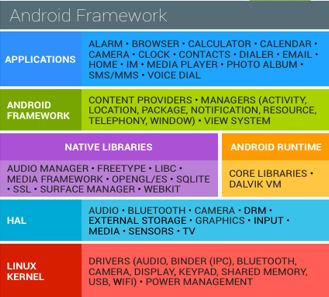
\includegraphics[width=\linewidth]{\figs\Capture1.JPG}
%  \caption{The Android Framework}
%  \label{fig:AndroidFramework}
%\end{figure}

\subsection{Before Android Marshmallow}
Before Android sdk 23, the permission model was based on a "do-or-die" concept. Users were given a list of permissions that would be required upon clicking the "install" link on an application on Google Play. There were no options to grant permissions selectively or revoke when not needed, and choosing not to grant a particular permission resulted in the application installation process being terminated\cite{felt2011effectiveness}. User choice was limited to whether they wanted to use the application, or not, and this has caused habituation even in later versions where permissions can be toggled\cite{wijesekera2015android}, since users choose to approve permissions by reflex as part of the installation process of an application. 
 
\subsection{After Android Marshmallow}

\section{Problems with the existing system}
The current permission model is problematic and offers loopholes that can be manipulated to compromise privacy of user data. This section will include a condensed view of research in this domain which highlight and offer solutions to some of these issues. 

\subsection{Least Privilege}
Both the most popular mobile operating systems, iOS and Android, require that developers follow the principle of "least privilege" with regard to permissions. The principle of least privilege states that "Every program and every user of the system should operate using the least set of privileges necessary to complete the job"\cite{schneider2004least}. In the context of Android applications, the principle states that developers should only ask for the very minimum of permissions that are required for the application to function\cite{enck2009understanding}. Applications on the Apple AppStore are screened to check adherence to this principle(and other factors) before being made available for download\cite{gilbert2011vision}. However since there is no such screening process for Android applications, research has shown that these permission guidelines are not generally adhered to by developers\cite{stevens2013asking}. Applications which do follow the permission guidelines are not necessarily popular with users, since permission requests either tend to be ignored due to lack of understanding\cite{felt2011android} \cite{kelley2012conundrum} or granted regardless of whether they are privacy sensitive or not due to habituation\cite{felt2012android}. This results in many popular applications not following the principle of least privilege\cite{wei2012permission}, with research showing that more than 33\% end up asking for more permissions than are required\cite{felt2011android}.

\subsection{Capability Leaks}
Applications can sometimes access permissions which are not requested at install time. Such violations of the permission architecture to access data are referred to as 'capability leaks' \cite{grace2012systematic} \cite{grace2011detecting}. A tool named Woodpecker, which analyzes each application to detect readability of permissions from unguarded interfaces, is frequently used in research in this domain \cite{zhou2012hey}. Through Woodpecker, two different types of capability leaks are identified; explicit leaks which find loopholes and access data without actually requesting permission and implicit leaks which let applications inherit permissions from another application, generally through intents. Other tools used to detect capability leaks include DroidChecker and IntentFuzzer \cite{yang2014intentfuzzer} \cite{chan2012droidchecker}. Capability leaks can also be exploited by malicious applications which use permissions which access permissions which have not been consiously granted to an application by a user for privilege escalation, using this to bypass restrictions on application functionality imposed due to the sand-boxing system\cite{davi2010privilege}.  

\subsection{Data Availability After Uninstallation}
Since application permissions once granted are not revoked even upon uninstallation of an application, the data collected through the permissions granted while the application was installed may still be accessible once the app is uninstalled. Upon uninstallation, the user identity belonging to the application is deleted, but the permissions allowed are not revoked, and data still exists as “orphans” without a unique identifier (or “parent”). These “orphans” may later be exploited by malware causing privacy breaches and leaking of sensitive data \cite{zhang2016life}. Users misunderstanding or choosing not to read permission requests before granting create lasting consequences, the effects of which continue to compromise privacy even after uninstallation of the problematic applications.

\subsection{Permission Creep}
Permission creep occurs in applications that do not follow the principle of least privilege and ask for extra permissions\cite{vidas2011curbing}. Applications may sometimes require permissions that are not required for the core functionality of the application, but rather due to revenue generation methods, since most 'free' applications available on the PlayStore require in-app purchases for extra functionality. Some of these 'free' and low cost applications may sell data to advertisers to generate revenue, without explicit permission from the user. Extra permissions may also be requested in cases where developers have difficulty trying to align permission requests with the functionality required for the application, resulting in genuinely having to request extra permissions that seems unnecessary on analysis, but are mandatory for certain functions \cite{vidas2011curbing}. For example an update for the popular game Angry Birds caused controversy by requesting permission to send SMS messages, which is not part of the expected functionality of the application. However Rovio (the company behind Angry Birds) later explained that this is due to the payment methodology needed to purchase new levels, where an SMS message is sent to Rovio from the device to be billed later by the carrier \cite{w} \cite{u}. 
\smallskip

Studies have shown that over 50\% of applications that request location access do so with the intent of sharing the information with advertisers for targeted marketing\cite{saint201050}. However, completely disallowing such requests would negatively impact the quality of applications available for Android since the revenue generation model would not survive. \cite{aa} In an ideal situation a user should be informed as to why an application is requesting a particular permission; as part of its core functionality, secondary functionality, as a method of revenue generation or any other usage for a permission to be requested. Research has shown that people tend to base their decisions on the reason behind data access\cite{lin2014modeling}. However this is not possible with the current model since the level of information made available to users regarding application permission requests is decided on by the developer.

\section{Proposed Solutions}
Apart from tools developed to identify and provide solutions to the issues discussed above, there have been several research related to alternate models or methodologies that could be followed to mitigate privacy risks in the current model.

\subsection{Facilitating Informed Decisions}
Researchers have suggested hierarchical solutions\cite{barrera2010methodology} and better breakdown of Android applications to create more fine-grained permission toggles\cite{bugiel2013flexible} as solutions to the problems caused by the do-or-die model in Android versions older than M. The current model does not allow users access to information as to why a particular permission is required, and studies have shown that this could be improved through analyzing human factors more effectively when allowing users to make these decisions, with personal examples and more privacy information having been proven to provide better understanding of permission requests and result in less breaches of privacy\cite{kelley2013privacy} \cite{harbach2014using}.  

\subsection{Code Analysis to Curb Permission Creep}
Applications requesting unecessary permissions and causing permission creep can be analyzed through static code analysis, by using tools such as pScout\cite{au2012pscout}, and FlowDroid\cite{arzt2014flowdroid}. Static code analysis generally involves reaing the Android Manifest and matching permissions which have been requested to those actually used by functions that provide core functionality of the application. Dynamic analysis of applications, runtime monitoring and Java code analysis have also been successful in identifying applications with permission creep \cite{spreitzenbarth2013mobile}. Context of a permission request; time of the request, whether the screen is on or off, whether the application is running visibly as a background or foreground application or service, what the device was displaying while the permission request was taking place, frequency of repitive permission requests(for example searching for network or wifi information) have been shown to influence users when deciding whether a particular permission request is appropriate \cite{wijesekera2015android}. This conforms to the Theory of Contextual Integrity\cite{nissenbaum2004privacy} with regard to privacy, since the context and flow contribute towards the attitude of a user towards a privacy sensitive request, and not just information such as usage, reason etc.

\subsection{User Driven Solutions}



\section{Transitivity of Trust}